\documentclass[12pt,twoside]{article}

%%%%%%%%%%%%%%%%%%%%%%%%%%%%%%%%%%%%%%%%%%%%%%%%%%%%%%%%%%%%%%%%%%%%%%%%%%%%%

% Definitions for the title page
% Edit these to provide the correct information
% e.g. \newcommand{\reportauthor}{Timothy Kimber}

\newcommand{\reporttitle}{Molecular dynamics simulations of the effect of trehalose on the stability of a copper-containing amino oxidase}
\newcommand{\reportauthor}{Pau Domínguez Sorribas}
\newcommand{\supervisor}{Jordi Villà Freixa}
\newcommand{\institution}{CBBL research group at UVic-UCC}
\newcommand{\degreetype}{Biotechnology}

%%%%%%%%%%%%%%%%%%%%%%%%%%%%%%%%%%%%%%%%%%%%%%%%%%%%%%%%%%%%%%%%%%%%%%%%%%%%%

% load some definitions and default packages
\usepackage[a4paper,hmargin=2.8cm,vmargin=2.0cm,includeheadfoot]{geometry}
\usepackage{textpos}
\usepackage{tabularx,longtable,multirow,subfigure,caption}%hangcaption
\usepackage{fancyhdr} % page layout
\usepackage{url} % URLs
\usepackage[english]{babel}
%\usepackage{afterpage}
\usepackage{amsmath}
\usepackage{amssymb}
\usepackage{systeme}
\usepackage{graphicx}
\usepackage{dsfont}
\usepackage{epstopdf} % automatically replace .eps with .pdf in graphics
%\usepackage{backref} % needed for citations
\usepackage{array}
\usepackage{latexsym}
\usepackage{lipsum}
\usepackage{tikz}
\usepackage{xcolor}
\usepackage{tabularx}
\usepackage{makecell}
\usetikzlibrary{angles, arrows.meta, quotes}
\usepackage[pdftex,hypertexnames=false,colorlinks]{hyperref} % provide links in pdf

\usepackage[skip=10pt plus1pt, indent=40pt]{parskip}

\hypersetup{pdftitle={},
  pdfsubject={}, 
  pdfauthor={},
  pdfkeywords={}, 
  pdfstartview=FitH,
  pdfpagemode={UseOutlines},% None, FullScreen, UseOutlines
  bookmarksnumbered=true, bookmarksopen=true, colorlinks,
    citecolor=black,%
    filecolor=black,%
    linkcolor=black,
    linkbordercolor=blue,%
    urlcolor=blue}

\usepackage[all]{hypcap}


%\usepackage{color}
%\usepackage[tight,ugly]{units}
%\usepackage{float}
%\usepackage{tcolorbox}
%\usepackage[colorinlistoftodos]{todonotes}
% \usepackage{ntheorem}
% \theoremstyle{break}
% \newtheorem{lemma}{Lemma}
% \newtheorem{theorem}{Theorem}
% \newtheorem{remark}{Remark}
% \newtheorem{definition}{Definition}
% \newtheorem{proof}{Proof}


%%% Default fonts
\renewcommand*{\rmdefault}{bch}
\renewcommand*{\ttdefault}{cmtt}



%%% Default settings (page layout)
\setlength{\parindent}{0em}  % indentation of paragraph

\setlength{\headheight}{14.5pt}
%\pagestyle{fancy}
%\renewcommand{\chaptermark}[1]{\markboth{\chaptername\ \thechapter.\ #1}{}} 

%\fancyfoot[ER,OL]{\sffamily\textbf{\thepage}}%Page no. in the left on odd pages and on right on even pages
%\fancyfoot[OC,EC]{\sffamily }
%\renewcommand{\headrulewidth}{0.1pt}
%\renewcommand{\footrulewidth}{0.1pt}
\captionsetup{margin=10pt,font=small,labelfont=bf}



% %--- chapter heading

\def\@makessectionhead#1{%
  \vspace*{10\p@}%
  {\parindent \z@ \raggedright \sffamily
    \interlinepenalty\@M
    \Huge\bfseries \thesection \space\space #1\par\nobreak
    \vskip 30\p@
  }}

% %---chapter heading for \chapter*  
\def\@makeschapterhead#1{%
  \vspace*{10\p@}%
  {\parindent \z@ \raggedright
    \sffamily
    \interlinepenalty\@M
    \Huge \bfseries  #1\par\nobreak
    \vskip 30\p@
  }}

\allowdisplaybreaks
%\usepackage[pages=all, color=black, position={current page.south}, placement=bottom, scale=1, opacity=1, vshift=5mm]{background}

% AMS Packages
\usepackage{amsmath}
\usepackage{amsthm}
\usepackage{amssymb}

% Unicode
\usepackage[utf8]{inputenc}
\usepackage{hyperref}
\hypersetup{
	unicode,
%	colorlinks,
%	breaklinks,
%	urlcolor=cyan, 
%	linkcolor=blue, 
	pdfauthor={Author One, Author Two, Author Three},
	pdftitle={A simple article template},
	pdfsubject={A simple article template},
	pdfkeywords={article, template, simple},
	pdfproducer={LaTeX},
	pdfcreator={pdflatex}
}


% Natbib
\usepackage[sort&compress,numbers,square]{natbib}
\bibliographystyle{unsrt}

\usepackage{graphicx, color}
\graphicspath{{figures/}}

\usepackage{mathrsfs} % for \mathscr command

\usepackage{orcidlink}

\usepackage{listings}
\newcommand{\R}[0]{\mathds{R}} % real numbers
\newcommand{\Z}[0]{\mathds{Z}} % integers
\newcommand{\N}[0]{\mathds{N}} % natural numbers
\newcommand{\C}[0]{\mathds{C}} % complex numbers
\renewcommand{\vec}[1]{{\boldsymbol{{#1}}}} % vector
\newcommand{\mat}[1]{{\boldsymbol{{#1}}}} % matrix
\lstset{ %
    basicstyle=\ttfamily\footnotesize,
    commentstyle=\color{ForestGreen},
    frame=single,
    keywordstyle=\color{black},
    language=Bash,
    showstringspaces=false,
    %morekeywords={blue},
    morestring=[s][\color{Gray}]{<}{>},
    morestring=[s][\color{OrangeRed}]{\ -}{\ },
    morestring=[s][\color{OrangeRed}]{*}{\ },
    morestring=[s][\color{OrangeRed}]{|}{\ },
    morestring=[s][\color{OrangeRed}]{\&}{\ },
}
\renewcommand{\lstlistingname}{Command}
%----------------------------------------------------------------------------------------


% load some macros
\input{notation}

\date{June 2024}

\begin{document}
\selectlanguage{english}

% load title page
\input{titlepage}


% page numbering etc.
\pagenumbering{roman}
\clearpage{\pagestyle{empty}\cleardoublepage}
\setcounter{page}{1}
\pagestyle{fancy}

%%%%%%%%%%%%%%%%%%%%%%%%%%%%%%%%%%%%


\begin{abstract}

This report delves into the molecular dynamics (MD) simulations of pea diamine oxidase (DAO) in the presence and absence of trehalose molecules, utilizing the AMBER software suite. The primary aim is to investigate the stabilizing effects of trehalose on DAO, an enzyme crucial for the metabolism of biogenic amines. DAO simulations are conducted in a truncated octahedral box with periodic boundary conditions to emulate an infinite system, enhancing the realism of the molecular environment. The study is ongoing, with preliminary results validating the MD simulations of trehalose molecules alone, ranging from one to twenty-five, in a cubic box. These initial simulations are crucial for establishing the parameters and behaviors of trehalose in isolation, providing a foundational understanding necessary for subsequent simulations involving DAO. The next phase of the study incorporates DAO into the simulation box with varying concentrations of trehalose, allowing for the exploration of trehalose's potential protective effects on the enzyme's structure and function. The anticipated outcomes include insights into how trehalose interacts at the molecular level with DAO, potentially revealing mechanisms through which trehalose exerts its stabilizing effects. This work aims to bridge the gap between experimental observations of trehalose-induced stabilization and the molecular-level details provided by MD simulations, ultimately contributing to the broader understanding of enzyme stabilization mechanisms by disaccharides.

\end{abstract}
\selectlanguage{catalan}
\begin{abstract}

Aquest informe descriu simulacions de dinàmica molecular (MD) de la diaminooxidasa (DAO) del pèsol en presència i absència de molècules de trehalosa, utilitzant la suite de programari AMBER. L'objectiu principal és investigar els efectes estabilitzadors de la trehalosa sobre DAO, un enzim crucial per al metabolisme de les amines biogèniques. Les simulacions de DAO es realitzen en una caixa octaèdrica truncada amb condicions de límit periòdiques per emular un sistema infinit, millorant el realisme de l'entorn molecular. L'estudi està en curs, amb resultats preliminars que validen les simulacions MD de molècules de trehalosa soles, que van d'una a vint-i-cinc, en una caixa cúbica. Aquestes simulacions inicials són crucials per establir els paràmetres i comportaments de la trehalosa de manera aïllada, proporcionant una comprensió bàsica necessària per a les simulacions posteriors que involucren DAO. La següent fase de l'estudi incorpora DAO a la caixa de simulació amb diferents concentracions de trehalosa, permetent l'exploració dels efectes protectors potencials de la trehalosa sobre l'estructura i la funció de l'enzim. Els resultats previstos inclouen informació sobre com la trehalosa interacciona a nivell molecular amb DAO, potencialment revelant mecanismes a través dels quals la trehalosa exerceix els seus efectes estabilitzadors. Aquest treball pretén salvar la bretxa entre les observacions experimentals de l'estabilització induïda per la trehalosa i els detalls a nivell molecular proporcionats per les simulacions de MD, contribuint finalment a la comprensió més àmplia dels mecanismes d'estabilització enzimàtica per part dels disacàrids.

\end{abstract}
\selectlanguage{english}

\clearpage
%%%%%%%%%%%%%%%%%%%%%%%%%%%%%%%%%%%%
\section*{Acknowledgments}
This work is dedicated to my family and friends whose unwavering support and encouragement have been an immense help throughout this journey. Also I want to thank CBBL colleagues that help me with any doubt I had and explained me with patience how to correct the errors I was making. In addition I want to thank CSUC for letting me use for the first time a supercomputer to run all my simulations.
Last but not least, I want to thank my supervisor Jordi, not only for giving me the opportunity to participate in this project which I enjoyed a lot doing the research and procedure while learning new things from a new field, but also for helping me and giving me advice all along the project.

\clearpage{\pagestyle{empty}}

%%%%%%%%%%%%%%%%%%%%%%%%%%%%%%%%%%%%
%--- table of contents
\fancyhead[RE,LO]{\sffamily {Table of Contents}}
\tableofcontents 
\clearpage{\pagestyle{empty}}
\pagenumbering{arabic}
\setcounter{page}{1}
\fancyhead[LE,RO]{\slshape \rightmark}
\fancyhead[LO,RE]{\slshape \leftmark}


%%%%%%%%%%%%%%%%%%%%%%%%%%%%%%%%%%%%
\section{Introduction}


The relevance of digestive health has increased significantly in recent years due to the growing interest in safe, all-natural ways to enhance wellness in general. In this regard, probiotics have become a well-liked and scientifically supported choice.  In addition, enzymes are a vital component that increases the effectiveness of these products since they catalyze a variety of biochemical events that are important for gut health and digestion.


\subsection{Background}
\subsubsection{Probiotics}

For some time now, the number of intestinal disease cases has been increasing year by year. In Spain alone, the number increases by 2.5\% annually. This rise is partly attributed to the increased use of antibiotics, immunosuppressive therapy, and irradiation, among other treatments, which may cause alterations in the composition and have an effect on the gastrointestinal (GI) flora\cite{Gupta2009}. To combat and prevent intestinal diseases, people have started consuming probiotics. But what exactly is a probiotic?

Probiotics consist of living microorganisms, such as bacteria and yeasts, that provide health benefits to the host when consumed. According to the first use of this term back in 1965 by Lilly and Stillwell, "probiotics" refer to substances secreted by one organism which stimulate the growth of another\cite{Gupta2009}. Probiotics are present in some fermented foods, added to certain food products, and available on the market as dietary supplements.

The growing interest in probiotics is driven by their potential to restore and maintain a healthy balance of gut flora, especially after disturbances caused by medical treatments or diseases. These beneficial microorganisms can enhance the intestinal microbial balance, support the immune system, and improve overall gut health. The increased popularity of probiotics underscores a proactive approach to managing gut health and preventing intestinal diseases.

To be considered as a probiotic, the product concerned must fulfill several requirements:
\begin{itemize}
    \item     High cell viability (resistance to low pH and acids)
  
    \item   Ability to persists in the intestine even if the probiotic cannot colonize the gut

    \item  Adhesion to the the gut epithelium to cancel the flushing effects of peristalsis

    \item  Capability to interact or send signals to immune cells associated with the gut

    \item  Non-pathogenic

    \item  Resistance to processing

    \item  Capability to influence local metabolic activity
\end{itemize}

% (Table \ref{tab:taulaprobiotic})


% \begin{table}
% \caption{Probiotic requirements}
% \label{tab:taulaprobiotic}
% \begin{tabular}{|c|}
%     \hline
%     \thead{\textbf{REQUIREMENTS}} 
%     \\
%     \hline
%     High cell viability (resistance to low pH and acids)
%     \\
%     \hline
%     Ability to persists in the intestine even if the probiotic cannot colonize the gut
%     \\
%     \hline
%     Adhesion to the the gut epithelium to cancel the flushing effects of peristalsis
%     \\
%     \hline
%     Capability to interact or send signals to immune cells associated with the gut
%     \\
%     \hline
%     Non-pathogenic
%     \\
%     \hline
%     Resistance to processing
%     \\
%     \hline
%     Capability to influence local metabolic activity
%     \\
%     \hline
%   \end{tabular}
% \end{table}



Lately, some enzymes are being used alongside probiotics, enhancing their effectiveness in preventing symptoms of bowel diseases. Depending on the enzyme added to the probiotic, the functionality can vary. For instance, adding the lactase enzyme can help counter lactose intolerance by breaking down lactose, making it easier for individuals to digest dairy products.
\\[10pt]
However, using enzymes with probiotics comes with potential drawbacks. One of the most significant issues is the risk of the enzyme being degraded faster than the probiotic can be consumed. This degradation can lead to a waste of material as the enzyme loses its functionality before it can exert its beneficial effects. Such a scenario is undesirable for companies, as it would be unprofitable and result in economic losses. Ensuring the stability and effectiveness of enzyme-probiotic combinations is therefore critical to maximizing their health benefits and maintaining profitability.

To address the degradation problem of enzymes in probiotics, a viable solution is to incorporate a disaccharide into the final product. Previous studies with carbohydrates have demonstrated that saccharides possess exceptional properties in helping biomolecules, such as proteins, preserve their native structures under harsh conditions and dehydration. Disaccharides, such as trehalose, are particularly effective in stabilizing proteins and enzymes, thereby extending their functional lifespan within probiotic formulations. This protective mechanism involves the formation of a protective layer around the enzyme, reducing the likelihood of degradation and maintaining the enzyme's activity over time. By integrating disaccharides into enzyme-probiotic products, manufacturers can enhance the stability and efficacy of these formulations, ensuring that the enzymes remain active and beneficial until consumption, ultimately improving the product's therapeutic potential and economic viability\cite{shao_trehalose_2019}.



\subsubsection{Our project}

In order to solve the degradation problem, those who are in charge of the development of the product, brought a possible and viable solution that consists on adding trehalose in the final product. Thanks to previous studies related with low-concentration trehalose solution it has been proven its efficiency as a protein stabilizer \cite{shao_trehalose_2019}. 
In addition to several experiments to find out which concentration of trehalose works better as a stabilizer and if it works properly, it was decided to complement them by a performance of molecular dynamics (MD) simulations of a system made of water, trehalose and DAO. 

The molecule on which this project is focused is diamine oxidase or DAO, also known as histaminase or amine oxidase, copper-containing,1. Generally speaking DAO is a group of enzymes that oxidise diamines like histamine. In this specific project we're studying DAO from \textit{Pisum sativum}(Figure \ref{fig:1KSI}). 

\begin{figure}[tb]
\centering
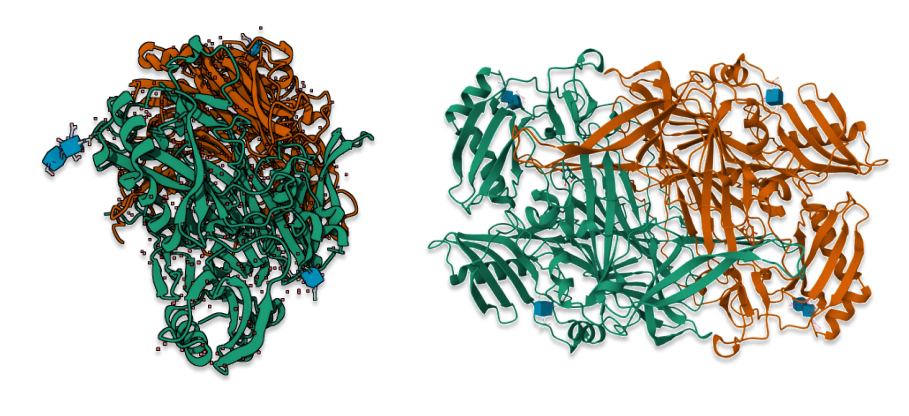
\includegraphics[width = 1\hsize]{./figures/1KSI}
\caption{3D conformation of Diamine Oxidase showing its homodimer structure (two identical chains in green and orange color) obtained by Re-Glyco from GlycoShape (left image) and 3D PDB viewer (right image)}
\label{fig:1KSI}
\end{figure}

Amine oxidation reaction is carried out by a cofactor callled 5-(2-carboxy-2-aminoethyl)-2-hydroxy-1,4-benzoquinone or topaquinone (TPQ), formed by post-translational modification of an invariant tyrosine residue \cite{Klinman2003}. It's evidenced that TPQ formation is given by self-processing mechanism which a tyrosine is oxidized by copper bounded to the protein and an oxygen. The reaction the amine catalyzes thanks to TPQ is:
\begin{equation}
    RCH_2NH_2 + H_2O + O_2 = RCHO + NH_3 + H_2O_2
\end{equation}

That reaction describe the oxidative deamination of polyamines, producing aminoaldehydes, hydrogen peroxide and ammonia during its process.

The formation of TPQ and the reaction happens thanks to the copper atom, which is located next to the active site. Due to its catalytic function DAO is involved in some physiological processes such as inflammation and immune response.  
Thanks to previous study, we know that DAO consists of a dimer of two crystallographically independent but chemically identical subunits, where each of them comprehends 3 domains; the largest of the three is a $\beta$-sandwich comprising two twisted anti-parallel $\beta$ sheets with eight and then strands respectively \cite{kumar_crystal_1996}. The smaller domains each, have two helices, then a four-stranded, anti-parallel, slightly curved b sheet with a $\beta$-hairpin turn in between strands 3 and 4. Those domains can be referred to as a "$\alpha/\beta$ roll" since they have the same topology and have very similar polypeptide folds at the first helix and the $\beta$ sheet. Regarding the second helix's orientation and connections, they are different.

There are numerous noteworthy features at the active site. It is buried, and getting to it from the substrate seems to involve a significant reorganization of the polypeptide. TPQ and the necessary Cu(II) atom are near to one another but not bonded; and the organic cofactor seems to be quite flexible.
In each subunit, the active site is located towards one edge of the $\beta$-sandwich domain D4 (the largest domain of the three) \cite{kumar_crystal_1996}.

DAO experiences interactions between its subunits, most of them between their largest domain, which occupies half of the molecular volume of the structure. If DAO exhibited interactions between residues on the arm of one subunit and the active site of the other one, being connected with an allosteric mechanism then it would be proved as other amine oxidases, but since for now it is not possible to confirm it, the network of intersubunit links close to the active site must have a different explanation.

A part from those interactions between the two largest domains of each subunit, there are also disulfide bridges between cysteine residues, but as they are far away from the active site, it is believed that they don't have an important role. For each subunit, two disulfide bridge are formed, that despite not having a mechanistic function, they might have an important structural role\cite{kumar_crystal_1996}.

In addition, DAO has four potential glycosilation sites which are located on the surface of the molecule is where NAG, which is a N-linked glycan.






\subsection{Molecular dynamics simulation of protein stability}
As we commented before, several simulations will be done, but how? First of all we have to understand what a molecular dynamics simulations is.
By Oxford Dictionary definition, a simulation consists in the "imitation of a situation or process" or "the action of pretending deception \cite{Katiyar2018}.
Although crystallographic studies clearly show the critical role that protein flexibility plays in ligand binding, the high cost and labor-intensive nature of producing them has pushed scientists to look for computational methods that can anticipate protein motions \cite{durrant_molecular_2011}. 

The fundamental concept of an MD simulation is simple. One may determine the force that each atom in a biomolecular system—such as a protein encircled by water and possibly a lipid bilayer—by knowing the locations of all of the other atoms in the system. Thus, it is possible to anticipate each atom's spatial position as a function of time using Newton's equations of motion. Specifically, one iteratively calculates the forces acting on each atom, steps through time, and uses the results to update the velocity and position of each atom. The resulting trajectory is essentially a three-dimensional movie that shows the system's atomic-level configuration at each time step of the simulation.\cite{hollingsworth_molecular_2018}

There are various reasons why these simulations are effective. Initially, they manage to record the position and mobility of each atom at all times, which is exceedingly challenging for any kind of experiment. Second, the parameters used in the simulation are well-defined and controllable: the starting protein conformation, the ligands attached to it, the presence of mutations or post-translational modifications, the other molecules in its surroundings, the protein's protonation state, the temperature, the voltage across a membrane, and so forth. The impacts of many different kinds of molecular disturbances can be identified by comparing simulations run under various settings/parameters.

A molecular mechanics force field model, which is suited to the outcomes of quantum mechanical computations and, usually, to specific experimental observations, is used to compute the forces in an MD simulation. A typical force field includes, for instance, spring-like terms that model the preferred length of each covalent bond and terms capturing numerous different forms of interatomic interactions, as well as terms that capture electrostatic (Coulombic) interactions between atoms. These force fields are essentially imprecise. Moreover, no covalent bonds form or break in a standard MD simulation. Studies of processes involving modifications to covalent bonds or molecules are commonly conducted using quantum mechanics/molecular mechanics (QM/MM) simulations, in which a portion of the system is described using QM calculations and the remaining portion by MD simulation. \cite{hollingsworth_molecular_2018}

By how molecular dynamics are presented, seems that they are foolproof methods and flawless, but they are not, in fact present limitations. The two principal challenges MD simulations present are the force fields used since they require further refinement and the high computational demands. Despite being limitations that may interfere with the course of the procedure, they do not represent a problem since can be sorted out.\cite{durrant_molecular_2011}

Drug research greatly benefits from molecular dynamics simulations and the insights they provide into protein motion, even though there are some limitations in current force fields and conformational sampling. Looking at a single protein conformation doesn't tell us much about its dynamics, just like a single photo of a runner doesn't reveal much about her stride. Techniques like NMR, X-ray crystallography, and homology modeling create static models that help us understand macromolecular structures. However, drug binding and molecular recognition are very dynamic processes. When a small molecule, like a drug (or ligand), approaches its target (like a receptor) in solution, it encounters a macromolecule in constant motion, not a fixed structure.

The detailed process in which is based on this project will be explained in the methodology section.

\clearpage
%%%%%%%%%%%%%%%%%%%%%%%%%%%%%%%%%%%%
\section{Hypothesis and Objectives}


\subsection{Hypothesis}


In this project our main goal is to demonstrate if trehalose can stabilize DAO or not, thus preventing it from degradation so the major hypothesis would be:
Could the addition of trehalose in DAO achieve a stabilization of it?.


\subsection{Objectives}

To check if the given hypothesis is accurate or not, the main objectives of this project to be achieved to study the effect of the addition of trehalose into the protein system in water, would be the following ones:

\begin{enumerate}
    \item Parameterize the protein, cofactors and 
    carbohydrate
    \item Run simulations of trehalose to verify its
    stabilization property
    \item Run simulation of only protein in a water
    system to use as a control to compare
    \item Run a final simulation of protein-carbohydrate
    in a water system
\end{enumerate}

Once all the objectives are done, the final objective will be to collect results, compare them, discuss them and draw a conclusion from that comparison.

\newpage

\clearpage
%%%%%%%%%%%%%%%%%%%%%%%%%%%%%%%%%%%%
\section{Results}

Once all the simulations are run, we have to collect all that data. In our case we have to bring the results given from CSUC to our local computer by ssh connection. 


\subsection{Trehalose simulaltions results}

In order to firstly verify that trehalose behaves as a stable molecule in a water system with same parameterization as the final simulation of DAO with NAG, ions and trehalose; 5 different simulations of different concentration of trehalose molecules were run roughly 100 ns each. The results given from production process that are more important for us to analyze are the trajectory ones (\texttt{*.nc}) and the initial product topology file from each tleap. To visualize that trajectory with an RMSD (Root Mean Square Deviation) the tool cpptraj was used. 

\begin{figure}
    \centering
    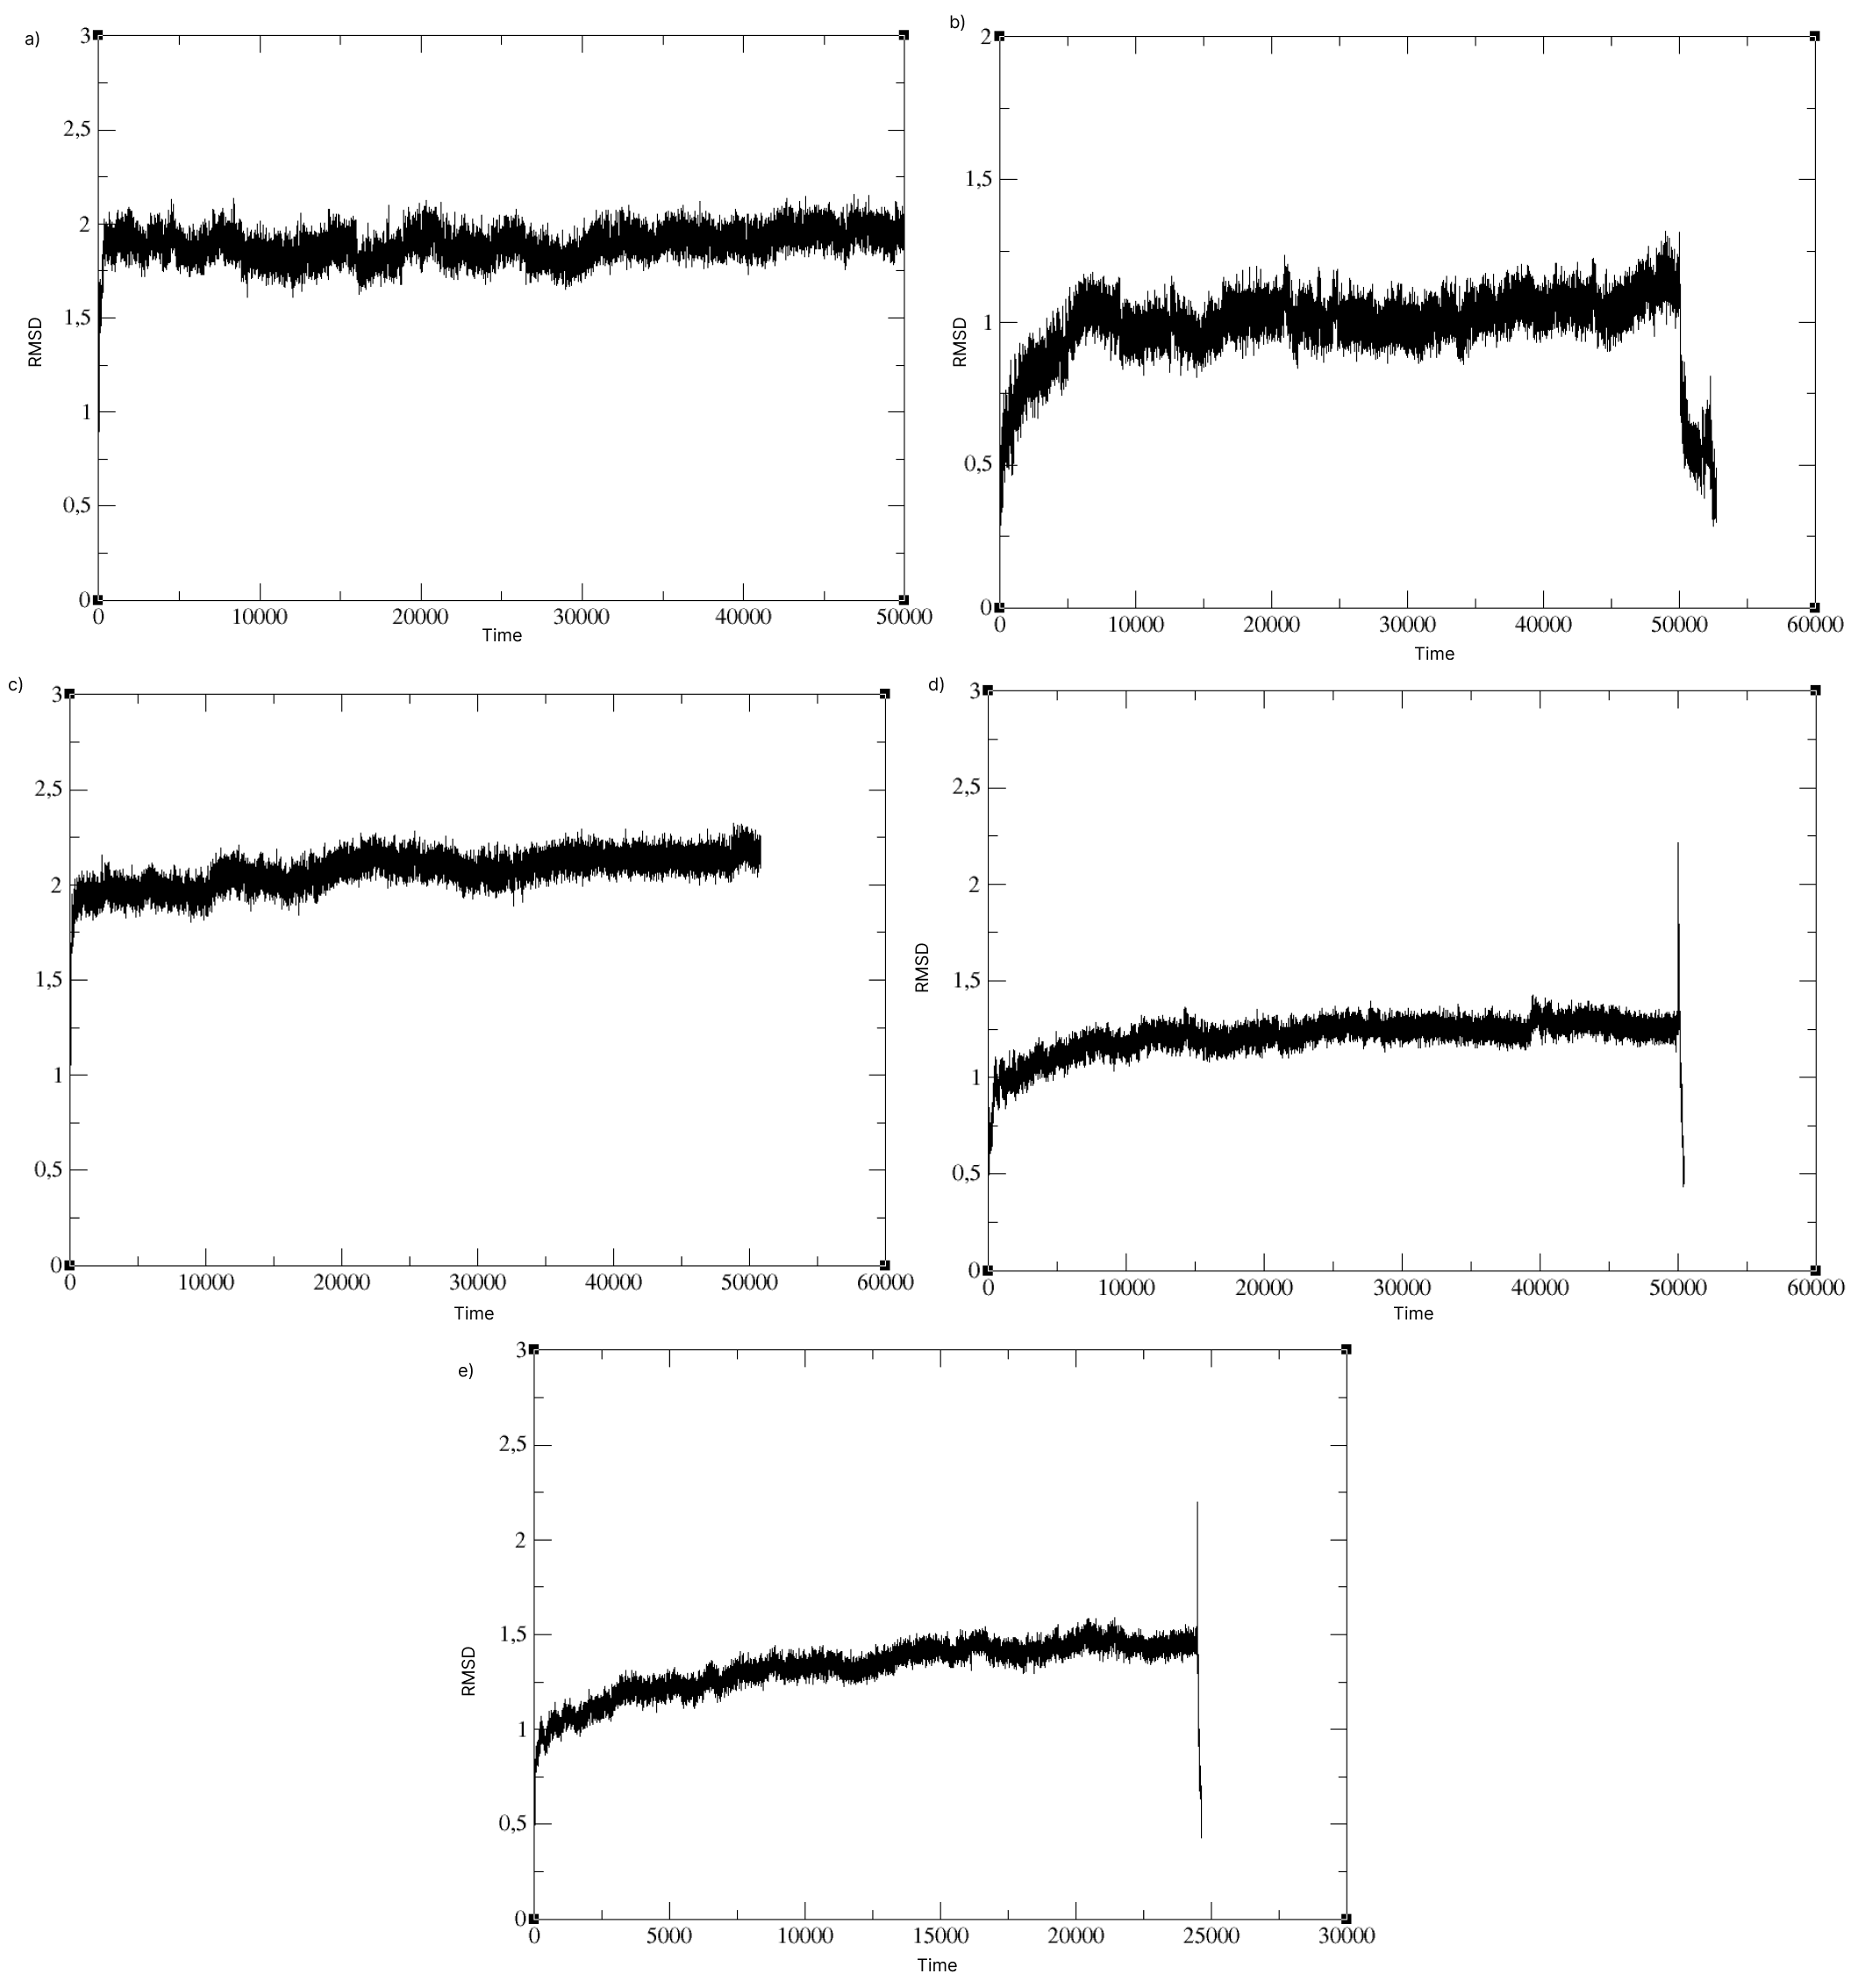
\includegraphics[width = 1\hsize]{./figures/rmsdtretot}
    \caption{Graphical representations of RMSD results from each of the trehalose simulations: a) 1 trehalose molecule, b) 2 trehalose molecules, c) 5 trehalose molecules, d) 10 trehalose molecules and e) 25 trehalose molecules.}
\label{fig:rmsdtre}
\end{figure}

Figure \ref{fig:rmsdtre} presents the Root Mean Square Deviation (RMSD) plots for five molecular dynamics (MD) simulations of trehalose molecules. Subfigures a, b, c, d, and e depict the RMSD trajectories for systems with 1, 2, 5, 10, and 25 trehalose molecules, respectively. All simulations were conducted for 100 ns, with the RMSD values stabilizing after an initial equilibration period. The plots indicate that each system maintained structural stability throughout the simulation duration, showcasing the consistent behavior of trehalose molecules in varying quantities under the simulated conditions. This stability is crucial for validating the reliability of the MD setup and a first indication of the appropriateness of the force field used to represent the disaccaride interactions.


\subsection{DAO without NAG, ions or trehalose in water system results}

After collecting all the data once the simulation was runned during 500 ns, it has to be prepared to be analyzed. Considering that each simulation result takes up a lot of space in the hard disk the the process must be carried out in an orderly and correct manner.
After trehalose results next results to be collected were those from DAO without NAG or trehalose simulation. Since the calculations took longer to be performed, the more runs were needed and therefore the size of each file. Due to this files size and the local computer used for this project which does not have a high storage capacity, the graphs created to visualize the results are from only some of the files (Figure \ref{fig:rmsdDAOnoNAG}). As it can be seen, even though the graphs are not made from all the files we can observe by the RMSD that the trehalose started to become unsettled. 



\begin{figure}
    \centering
    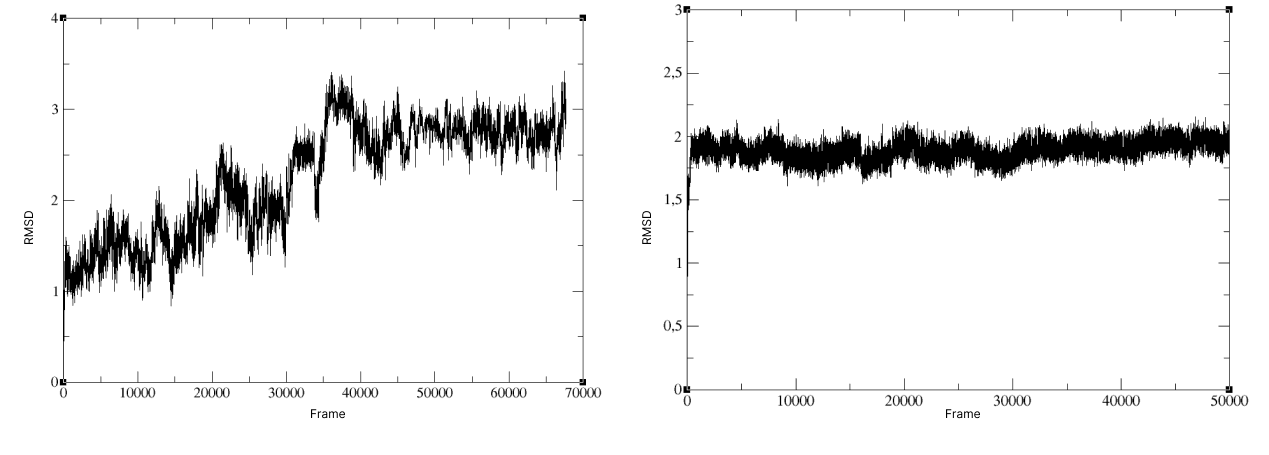
\includegraphics[width = 1\hsize]{./figures/rmsdmd1}
    \caption{Two RMSD graphs from the first four runs of the simulation (left image) and the first run of the simulation (right image) showing the measure of the average distance between the atoms}
    \label{fig:rmsdDAOnoNAG}
\end{figure}


\subsection{DAO with NAG and trehalose results}

The simulation which was going to be used, could not be realized. During the process of preparation of files everything was running as it was expected, except when the problems started once the tleap file was attempted to be run.
As the simulation could not be performed, there are no results to be analyzed and compared to previous ones.

\clearpage
%%%%%%%%%%%%%%%%%%%%%%%%%%%%%%%%%%%%
\section{Discussion}




Before analyzing the results shown in the previous section, it is necessary to take into account that we did not have results from the last simulation consisting of a system made of DAO, NAG and trehalose into a cubic water box, so instead of making a comparison between the results we have to make an assumption based on previous studies about what the results would be.

Our goal in this experiment was to investigate the stabilizing effects of trehalose on diamine oxidase (DAO) using molecular dynamics simulations. Our aim was to examine how the structural stability and functional dynamics of DAO were affected by varying trehalose concentrations. Our aim was to get deeper insight into the molecular interactions and mechanisms that result in the stability of the enzyme by simulating DAO in the presence of different amounts of trehalose molecules. The stability of enzymes for use in a variety of biotechnological and medical applications may be improved by the findings of this study.

Due to time and computer power constraints, we adapted the initial plan to focus on specific simulations. We conducted five molecular dynamics simulations, each with a different number of trehalose molecules (1, 2, 5, 10, and 25). These simulations were performed in a cubic box with periodic boundary conditions over a duration of 100 ns. This approach allowed us to gather comprehensive data on the behavior of trehalose molecules and their interactions under various concentrations, while managing computational resources effectively.

According to our trehalose simulations, trehalose molecules are consistently stable at various concentrations. For the duration of the 100 ns simulation, all systems—which had one to twenty-five trehalose molecules—maintained their structural integrity. Trehalose molecules rapidly adopted a stable conformation and hold it, as shown by the RMSD plots, indicating the robustness of the force fields and molecular dynamics setup. These results highlight trehalose's ability to function as a stabilizing agent in a range of molecular settings.

With regard to DAO, we have carried out an initial simulation of the enzyme  in the absence of trehalose. The RMSD analysis indicates that DAO maintains its native conformation over the course of the simulations, which provides an initial useful result that we plan to compare in future analysis with the same simulations carried out in presence of trehalose. Future research could investigate the optimal concentrations and combinations of trehalose with other protective agents to maximize stability and functionality. Additionally, experimental validation of these findings could pave the way for new formulations of enzyme-based products, improving their resilience and performance in real-world applications.

\clearpage
%%%%%%%%%%%%%%%%%%%%%%%%%%%%%%%%%%%%
\section{Conclusions}

The research carried out intended to replicate the fact that of disaccharides, particularly trehalose, in stabilizing enzymes within probiotic formulations, as has been shown before\cite{shao_trehalose_2019}. By incorporating trehalose into these products, the study aimed at demonstrating lower dynamical behavior of the protein, which one could link to a more stable system. In the initial proposal, we hypothesized that such stabilization may lead to a lower exposure of different domains and motifs of the protein to degradation. Unfortunately, the difficulty to access proper computational resources in available time and processing units (AMBER is well known to work fast in GPU-based computers, of which we had only a limited access to the CSUC supercomputing facilities), prevented us to advance beyond the first steps of our proposed molecular simulations runs. 

In addition, our analysis restrict to the exploration of the RMSD trends along the several simulations, and we have not succeeded in further analyses including root mean square fluctuations (RMSF) or the building of Markov models to analyze the free energy landscapes of DAO in the presence and absence of trehalose. However, and despite the limitations of our aproach, the molecular dynamics simulations carried out up to this moment provide enough sampling for further exploring such analytical tools, which pave the way to discuss possible outcomes with our industrial partner.

We suspect that the trehalose mediated DAO stabilization ensures that the enzyme remain functional until consumption. Formulations that include protective agents like trehalose can thus preserve the integrity and functionality of enzymes under various conditions.

Moreover, the study emphasizes the economic benefits of using disaccharides in enzyme-probiotic products. By preventing premature enzyme degradation, manufacturers can reduce material waste and improve the profitability of their products. This approach aligns with the need for cost-effective solutions in the health and wellness industry, where maintaining product efficacy is essential. The successful application of disaccharides to stabilize enzymes opens new avenues for developing more robust and reliable probiotic formulations, ultimately benefiting both consumers and manufacturers by delivering more consistent and effective health outcomes.

\section{Disclosure}

This project is part of the collaboration between the Computational Biochemistry and Biophyscis Lab and a biotechnology company that is currently producing the formulations of the trehalose stabilized diamine oxidase. The GitHub link including all the scripts and input files used in this work is available (under embargo due to the signed non-disclosure agreement between the university and the company) in \url{https://github.com/pauds01/TFG_DAO}. 

\clearpage
\section{References}

%%%%%%%%%%%%%%%%%%%%%%%%%%%%%%%%%%%%

%% bibliography
% https://libguides.usask.ca/bibtex/cite-latex
\bibliography{references.bib}
\bibliographystyle{plain}
\nocite{aduri_amber_2007}
\nocite{zuegg_molecular_2000}
\nocite{chong_protein-protein_2021}
\nocite{bryce_carbohydrate-protein_2001}
\nocite{king_molecular_2019}
\nocite{bohne-lang_glyprot_2005}
\nocite{bohm_glycosciencesdb_2019}
\nocite{floris_copper_2009}
\nocite{mcgrath_structure_2009}
\nocite{bohne-lang_glyprot_2005}
\nocite{danne_doglycanstools_2017}
\nocite{zhang_combination_2021}
\nocite{wu_variation_2021}
\nocite{wood1984spelunking}
\nocite{whitmore_constructing_2020}
\nocite{wells_mapping_2002}
\section{Annexes}
\subsection{Github}
\label{sub:github}
%%%%%%%%%%%%%%%%%%%%%%%%%%%%%%%%%%%%
Every complementary program or file is shared by a \href{https://github.com/pauds01/TFG_DAO}{Github} link where they are located in different folders depending on their use.
\end{document}
